\documentclass[]{AVSSimReportMemo}
\usepackage{AVS}
\usepackage{colortbl}


\newcommand{\ModuleName}{hillPoint}
\newcommand{\subject}{Guidance Module for Hill Frame Pointing}
\newcommand{\status}{Initial Version}
\newcommand{\preparer}{M. Cols}
\newcommand{\summary}{Generate the attitude reference to perform a constant pointing towards a Hill frame orbit axis}


\begin{document}

\makeCover


%
%	enter the revision documentation here
%	to add more lines, copy the table entry and the \hline, and paste after the current entry.
%
\pagestyle{empty}
{\renewcommand{\arraystretch}{2}
\noindent
\begin{longtable}{|p{0.5in}|p{4.5in}|p{1.14in}|}
\hline
{\bfseries Rev}: & {\bfseries Change Description} & {\bfseries By} \\
\hline
Draft & initial copy & M. Cols \\
\hline

\end{longtable}
}

\newpage
\setcounter{page}{1}
\pagestyle{fancy}

\tableofcontents
~\\ \hrule ~\\

\section{Module Input and Output}
Table \ref{tab:inputNavTable} shows the input message from the navigation system.
\begin{table}[h!]
	\centering
	\caption{Input Navigation Message}
	\begin{tabular}{|l|l|l|p{3in}|}
		\hline
		\rowcolor{BrickRed}
		\textcolor{white}{Name} & \textcolor{white}{Type} &
		\textcolor{white}{Length} &
		\textcolor{white}{Description}  \\ \hline
		$\bm{R}_S$ & double [] & 3 &
		Position vector of the spacecraft body-point with respect to the inertial frame in inertial frame components
		($\leftexp{N}{\bm{r}}_{B/N}$) . \\ \hline
		$\bm{v}_S$ & double [] & 3 &
		Velocity vector of the spacecraft point with respect to the inertial frame in inertial frame components
		($\leftexp{N}{\bm{v}}_{B/N}$). \\ \hline
	\end{tabular}
	\label{tab:inputNavTable}
\end{table}

Table \ref{tab:inputCelTable} shows the input message from Spice about the main celestial body.
\begin{table}[h!]
	\centering
	\caption{Input Spice Planet Message}
	\begin{tabular}{|l|l|l|p{3in}|}
		\hline
		\rowcolor{BrickRed}
		\textcolor{white}{Name} & \textcolor{white}{Type} &
		\textcolor{white}{Length} &
		\textcolor{white}{Description}  \\ \hline
		$\bm{R}_P$  & double [] & 3 &
		Position vector of the main celestial object with respect to the inertial frame in inertial frame components . \\ \hline
		$\bm{v}_P$  & double [] & 3 &
		Velocity vector of the main celestial object with respect to the inertial frame in inertial frame components . \\ \hline
	\end{tabular}
	\label{tab:inputCelTable}
\end{table}

Table \ref{tab:outputTable} shows the Attitude Reference output message of the module Hill Point.
\begin{table}[h!]
	\centering
	\caption{Output Attitude Reference Message}
	\begin{tabular}{|l|l|l|p{3in}|}
		\hline
		\rowcolor{BrickRed}
		\textcolor{white}{Name} & \textcolor{white}{Type} &
		\textcolor{white}{Length} &
		\textcolor{white}{Description}  \\ \hline
		$\sigma_{R/N}$ & double [] & 3 &
		MRP attitude set of the reference frame with respect to the reference. \\ \hline
		$\leftexp{N} \omega_{R/N}$ & double [] & 3 &
		Angular rate vector of the reference frame with respect to the inertial expressed in inertial frame components. \\ \hline
		$\leftexp{N} {\dot{\omega}_{R/N}}$ & double [] & 3 &
		Angular acceleration vector of the reference frame with respect to the inertial expressed in inertial frame components. \\ \hline
	\end{tabular}
	\label{tab:outputTable}
\end{table}
\newpage

\section{Hill Frame Definition}
The Hill reference frame takes the spacecraft's orbital plane as the principal one and has origin in the centre of the spacecraft. It is defined by the right-handed set of axes $\mathcal{H}:\{ \hat{\bm\imath}_{r}, \hat{\bm\imath}_{\theta}, \hat{\bm\imath}_{h} \}$, where\par
$\hat {\bm\imath}_{r}$  points radially outward in the direction that connects the center of the planet with the spacecraft. \par
$\hat {\bm\imath}_{h}$ is defined normal to the orbital plane in the direction of the angular momentum. \par
$\hat {\bm\imath}_{\theta}$ completes the right-handed triode.
\begin{figure}[htb]
	\centerline{
	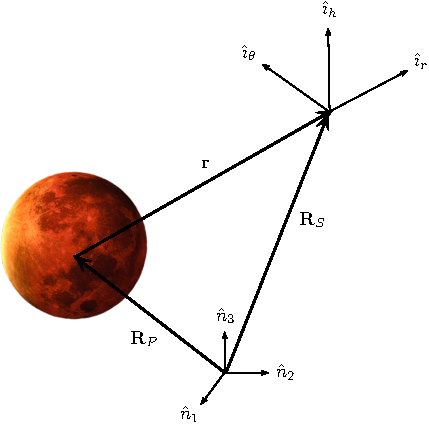
\includegraphics{Figures/Fig2}
	}
	\caption{Illustration of the Hill orbit frame $\mathcal{H}:\{ \hat{\bm\imath}_{r}, \hat{\bm\imath}_{\theta}, \hat{\bm\imath}_{h} \}$, and the inertial frame $\mathcal{N}:\{ \hat{\bm n}_{1}, \hat{\bm n}_{2}, \hat{\bm n}_{3} \}$.}
	\label{fig:Fig1}
\end{figure}


\section{Introduction}
In this module, the output reference frame $\mathcal{R}$ is to be aligned with the Hill reference frame $\mathcal{H}$. Note that the presented technique does not require the planet-fixed  frame to coincide with the inertial frame $\mathcal{N}:\{ \hat{\bm n}_{1}, \hat{\bm n}_{2}, \hat{\bm n}_{3} \}$. Figure 1 illustrates the general situation in which $\bm{R}_{s}$ is the position vector of the spacecraft with respect to the inertial frame and $\bm{R_{p}}$ is the position vector of the  celestial body with respect to the inertial frame as well.
The relative position of the spacecraft with respect to the planet is obtained by simple subtraction:
\begin{equation}
	\label{eq:r}
	\bm r = \bm R_{s} -  \bm R_{p}
\end{equation}
The same methodology is applied to compute the relative velocity vector:
\begin{equation}
	\label{eq:v}
	\bm v = \bm v_{s} -  \bm v_{p}
\end{equation}
Note that the position and velocity vectors of the spacecraft and the celestial body, $\bm{R}_S$,  $\bm{R}_P$,  $\bm{v}_S$ and  $\bm{v}_P$ are the only inputs that this module requires. Having $\bm r$ and $\bm v$, the Hill frame orientation is completely defined:
\begin{subequations}
	\begin{equation}
	\hat{\bm\imath}_{r} = \frac{\bm r}{r}
	\end{equation}
	\begin{equation}
	\hat{\bm\imath}_{h} = \frac{\bm{r}\times{\bm{v}}}{r v}
	\end{equation}
	\begin{equation}
	\hat{\bm\imath}_{\theta} = \hat{\bm\imath}_{h} \times \hat{\bm\imath}_{r}
	\end{equation}
\end{subequations}
And the Direction Cosine Matrix to map from the reference frame to the inertial is obtained:
\begin{equation}
	[RN] =  \begin{bmatrix}
       		\hat{\bm\imath}_{r} \\
		\hat{\bm\imath}_{\theta} \\
		\hat{\bm\imath}_{h}
      \end{bmatrix}
\end{equation}
The corresponding MRP attitude set is computed using the following function from the Rigid Body Kinematics library of Reference~\citenum{schaub}:
$$ [RN] = \textrm{C2MRP}(\bm\sigma_{R/N})$$

\section{Angular Velocity Descriptions}
Let $\mathcal{R}_{0}$ reference the Hill orbit frame. The orbit frame angular rate and acceleration vectors are given by
\begin{equation}
	\label{eq:omega_R0}
	\bm\omega_{R_{0}/N} = \dot f \hat{\bm\imath}_{h}
\end{equation}
\begin{equation}
	\label{eq:domega_R0}
	\dot{\bm\omega}_{R_{0}/N} = \ddot f \hat{\bm\imath}_{h}
\end{equation}
where $f$ is the true anomaly, whose variation is determined through the general standard astrodynamics relations:
\begin{align}
  \dot f &= \frac{h}{r^{2}}
  \\
  \ddot f &= - 2 \frac{\bm v \cdot \hat{\bm\imath}_{r}}{r} \dot f
\end{align}
The angular rate $\bm\omega_{R/N}$ and acceleration $\dot{\bm\omega}_{R/N}$ of the output reference frame $\mathcal{R}$  still need to be computed.
Since the desired attitude is a fixed-pointing one, $\mathcal{R}$ does not move relative to $\mathcal{R}_{0}$. Thus, the angular velocity of the reference frame happens to be
\begin{equation}
	\label{eq:omega_R}
	\bm\omega_{R/N} = \bm\omega_{R/R_{0}} + \bm\omega_{R_{0}/N} = \dot{f} \hat{\bm\imath}_{h}
\end{equation}
Again, given that $ \hat{\bm\imath}_{h}$ is fixed as seen by the reference frame $R$,  the acceleration vector of the reference frame expressed in the reference frame simply becomes:
\begin{equation}
	\label{eq:domega_R}
	\dot\omega_{R/N} = \ddot{f} \hat{\bm\imath}_{h}
\end{equation}
Both $\bm\omega_{R/N}$ and $\dot\omega_{R/N} $ need to be expressed in the inertial frame $N$. \newline
Given
\begin{subequations}
\begin{equation}
\leftexp{R}{\bm \omega_{R/N} } =
      \begin{bmatrix}
       0\\ 0 \\ \dot{f}
      \end{bmatrix}
\end{equation}
\begin{equation}
 \leftexp{R}{\bm\dot{\omega}_{R/N}  } =
      \begin{bmatrix}
       0\\ 0 \\ \ddot{f}
      \end{bmatrix}
\end{equation}
\end{subequations}
Then,
\begin{subequations}
\begin{equation}
	\leftexp{N} {\bm{\omega}_{R/N}} =  [NR] \textrm{ } \leftexp{R} {\bm\omega_{R/N} }
\end{equation}
\begin{equation}
	\leftexp{N} {\bm\dot{\omega}_{R/N} }=[NR] \textrm{ } \leftexp{R} {\bm\dot{\omega}_{R/N}}
\end{equation}
\end{subequations}
Where $ [NR] = [RN]^T$.




\bibliographystyle{unsrt}
\bibliography{references}

\end{document}
